\documentclass{article}
\usepackage{amsmath}
\usepackage{amssymb}
\usepackage{graphicx}
\usepackage[margin=1in]{geometry}
\usepackage{hyperref}
\usepackage{caption}
\usepackage{float}
\graphicspath{{images/}}
\hypersetup{
  colorlinks=true,
  urlcolor=blue,
}
\begin{document}

\title{A Projection}
\author{Aresh Pourkavoos}
\maketitle

\[
Q =
\frac{1}{2\sqrt{2+\varphi}}
\begin{pmatrix}
  \varphi & \varphi & 1 & -1 & 0 & 0 \\
  1 & -1 & 0 & 0 & \varphi & \varphi \\
  0 & 0 & \varphi & \varphi & 1 & -1 \\
  -1 & -1 & \varphi & -\varphi & 0 & 0 \\
  \varphi & -\varphi & 0 & 0 & -1 & -1 \\
  0 & 0 & -1 & -1 & \varphi & -\varphi
\end{pmatrix}
\]

The $6 \times 6$ matrix above is orthonormal,
meaning that it represents a rotation of 6-dimensional space.
$\varphi$ is the golden ratio $\frac{1+\sqrt{5}}{2}$,
the positive solution to the equation $\varphi^2 = \varphi+1$.
I found it while exploring the Penrose tiling(s)
and the mathematical theory behind it,
which I hope to summarize here.

Although Roger Penrose has multiple related aperiodic tilings in his name,
When I mention ``the'' Penrose tiling, I refer to the one made of two golden rhombi,
known as the P3 tiling.
However, even this is insufficient to narrow it down,
as depending on the method of construction,
there might be uncountably many variations of P3.
Rather than get bogged down in definitions too early on,
``the'' Penrose tiling is this one:

[Image]

It has at least four different properties
which either uniquely determine or narrow down its construction:
\begin{itemize}
\item
  The tiles may have ``matching rules'' enforced,
  where the edges are given a type and an orientation
  which much match between adjacent tiles.
\item
  The tiling may be produced by a ``substitution rule,''
  which begins with a small construction of rhombi
  and repeatedly splits them into smaller and smaller pieces.
\item
  It can be obtained as the dual of a ``pentagrid,''
  an arrangement of 5 sets of parallel lines in the plane.
\item
  It can arise from a ``cut and project'' scheme,
  which involves taking a slice of a 5-dimensional cubic grid.
\end{itemize}

First, the matching rules are visualized below.
\begin{center}
  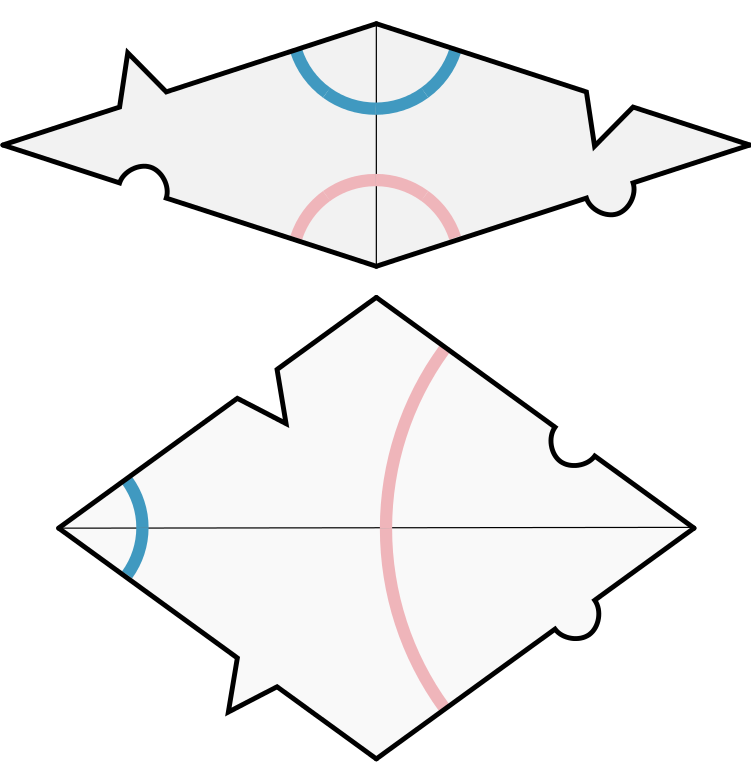
\includegraphics[width=0.25\linewidth]{matching.png}\\
  Source: \href{https://en.wikipedia.org/wiki/User:Geometry_guy}{Geometry guy}
  at \href{https://en.wikipedia.org/wiki/}{English Wikipedia}
\end{center}
The rhombi in a Penrose tiling (of type P3)
must be able to be replaced with the modified rhombi above and still fit together.
These rules prevent the rhombi from tiling periodically, as below.
\begin{center}
  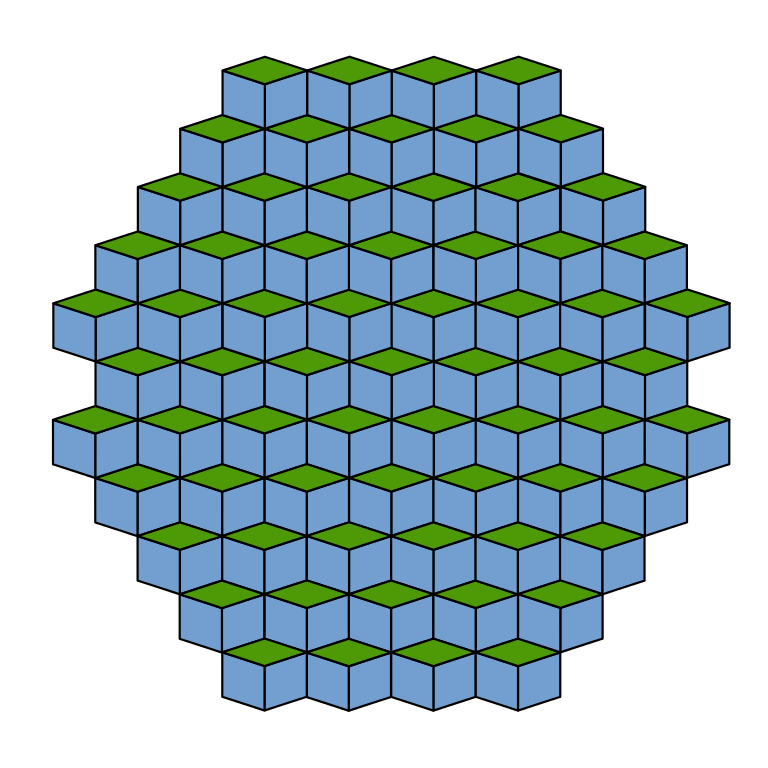
\includegraphics[width=0.25\linewidth]{periodic.png}\\
  Source: \href{https://en.wikipedia.org/wiki/User:Geometry_guy}{Geometry guy}
  at \href{https://en.wikipedia.org/wiki/}{English Wikipedia}
\end{center}

There are an infinite number of tilings that follow these rules,
but they are all locally indistinguishable;
that is, any contiguous ``patch'' of rhombi
found within any tiling
is also contained within every other tiling -
an infinite number of times!

Next, the tiling may be formed by substitution rules.
It is easier to describe these rules
when the tiles are not rhombi but half-rhombi,
where the tiles are cut along the diagonals
marked in the image showing the matching rules.
They become isoceles triangles
whose sides are in golden ratio to each other,
known as the Robinson triangles.

\end{document}
